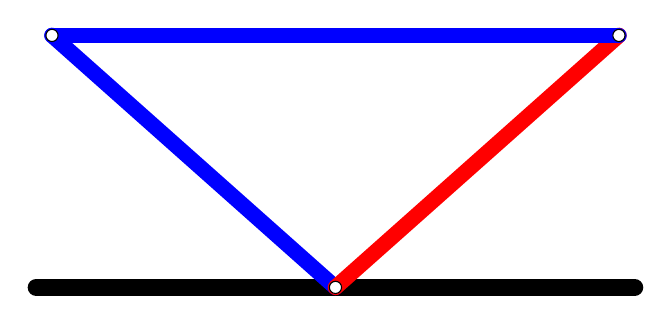
\begin{tikzpicture}[line cap=round]
  % Thickness parameters
  \def\edgeW{5.6pt}   % colored edges
  \def\groundW{6.2pt} % ground strip

  % Key points
  \coordinate (G) at (0,0);        % ground junction
  \coordinate (L) at (-3.6,3.2);   % top-left node
  \coordinate (R) at ( 3.6,3.2);   % top-right node

  % Ground (black)
  \draw[line width=\groundW] (-3.8,0) -- (3.8,0);

  % Stalks (left blue, right red)
  \draw[blue, line width=\edgeW] (G) -- (L);
  \draw[red,  line width=\edgeW] (G) -- (R);

  % Top bar (blue)
  \draw[blue, line width=\edgeW] (L) -- (R);

  % Nodes (white filled circles with thin black outline)
  \foreach \p in {L,R,G}{
    \filldraw[fill=white, draw=black, line width=0.4pt] (\p) circle[radius=2.2pt];
  }
\end{tikzpicture}